\documentclass[12pt,a4paper]{article}
\usepackage[utf8]{inputenc}
\usepackage[american]{babel}
\usepackage{amsmath}
\usepackage{amsfonts}
\usepackage{amssymb}
\usepackage{mathtools}
\DeclarePairedDelimiter{\abs}{\lvert}{\rvert}
\newcommand{\pdiff}[2]{\frac{\partial #1}{\partial #2}}
\newcommand{\pdiffn}[3]{\frac{\partial^{#3} #1}{\partial #2^{#3}}}
\usepackage{geometry}
\usepackage[square]{natbib}
\usepackage[bookmarks,hidelinks]{hyperref}
\usepackage{subfiles}
\usepackage[numbib,nottoc]{tocbibind}
\usepackage{url}
\usepackage{todonotes}
\usepackage{siunitx}
\usepackage{listings}
\usepackage{color}
\lstset{
  language=Python,
  keywordstyle=\bfseries\ttfamily\color[rgb]{0,0,1},
  identifierstyle=\ttfamily,
  commentstyle=\color[rgb]{0.133,0.545,0.133},
  stringstyle=\ttfamily\color[rgb]{0.627,0.126,0.941},
  showstringspaces=false,
  basicstyle=\small,
  numberstyle=\footnotesize,
  numbers=left,
  stepnumber=5,
  numberfirstline=true,
  breaklines=true,
  breakatwhitespace=false,
  frame=single,
%  morekeywords={sumsq, randi}
}
\usepackage{tikz}
\usetikzlibrary{patterns}
\renewcommand{\epsilon}{\varepsilon}
\usepackage{titling}
\newcommand{\subtitle}[1]{
  \posttitle{
    \par\end{center}
    \begin{center}\large#1\end{center}
    \vskip0.5em}
}
\author{Marc John Bordier Dam}
\title{Using Numerical Methods to Explore Quantum Mechanics}
\linespread{1.3}

\begin{document}
\selectlanguage{american}
\maketitle

\section{Summary}
\todo[inline]{WRITE ME!}

\section{Introduction}
\todo[inline]{WRITE ME!}

\section{Schrödinger's Equation and its Solutions}
The most fundamental equation in quantum mechanics is the Schrödinger equation. It governs which functions are worthy of study, that is, which functions are allowed wave functions in a given potential. The time-dependent Schrödinger equation in one dimension is
\begin{equation}
i \hbar \pdiff{\Psi}{t} = - \frac{\hbar^2}{2 m} \pdiffn{\Psi}{x}{2} + V \Psi.
\end{equation}
To make solving the time-dependent Schrödinger equation easier we use separation of variables to obtain the time-independent Schrödinger equation
\begin{equation}
- \frac{\hbar^2}{2 m} \pdiffn{\psi}{x}{2} + V \psi = E \psi,
\end{equation}
where $\Psi = \psi e^{-\frac{i E t}{\hbar}}$.

The wave functions which are solutions to the time-independent Schrödinger euqation represent stationary states. These stationary states have the nice property that any function in Hilbert space can be written as a linear combination of them. Thus it is in many cases sufficient to work with the stationary states and linear combinations of them. Below we will present the stationary states along with their allowed energies for the infinite and finite square well.

\subsection{The Infinite Square Well}
\begin{figure}
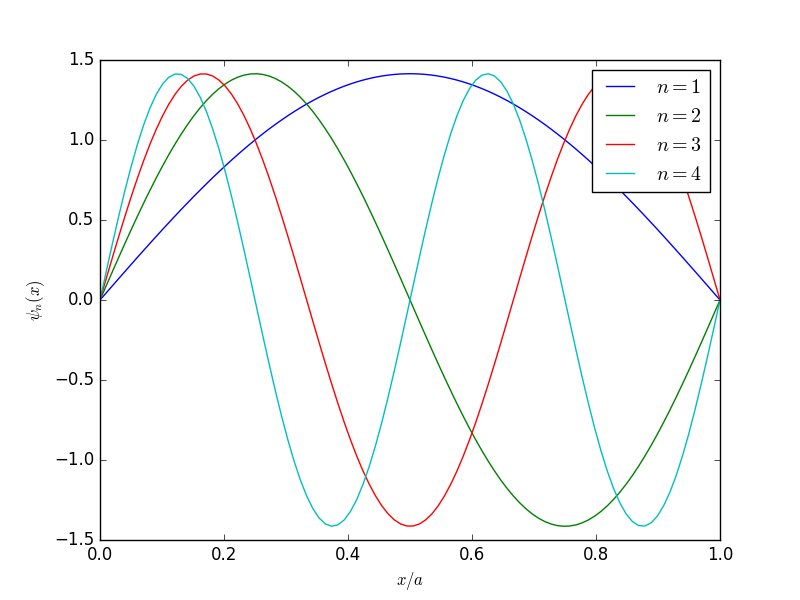
\includegraphics[width=\textwidth]{../Python/ISW_stationarySolutions.png}
\caption{Wave Functions in the Infinite Square well}
\label{fig:infiniteSquareWell}
\end{figure}

In the infinite square well the potential is given by
\begin{equation}
V = \begin{cases} 0, & 0 \leq x \leq a \\
                  \infty, & \text{otherwise} \end{cases}.
\end{equation}

Outside the well the wave function is $0$ and inside the well it is given by
\begin{equation}
\psi_n(x) = \sqrt{\frac{2}{a}} \sin \left( \frac{n \pi}{a} x \right),
\end{equation}
where $n$ is any positive integer. In the infinite square well the energy spectrum is discrete with the $n$th stationary state having the energy
\begin{equation}
E_n = \frac{n^2 \pi^2 \hbar^2}{2 m a^2}.
\end{equation}
Some of the wave functions are shown in figure~\ref{fig:infiniteSquareWell}.

\subsection{The Finite Square Well}
\begin{figure}
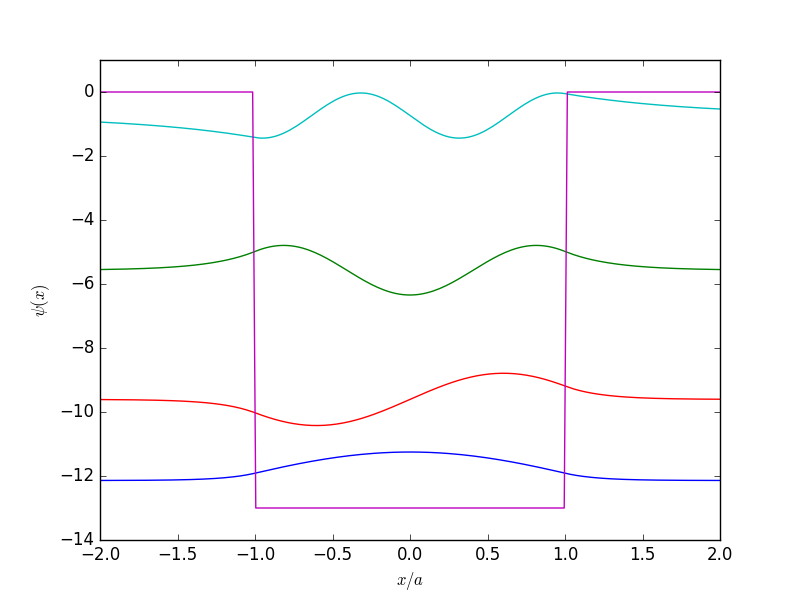
\includegraphics[width=\textwidth]{../Python/FSW_boundStates.png}
\caption{Wave Functions in the Finite Square well}
\label{fig:finiteSquareWell}
\end{figure}

In the finite square well the potential is given by
\begin{equation}
V = \begin{cases} -V_0, & -a \leq x \leq a \\
                  0, & \text{otherwise} \end{cases},
\end{equation}
where $V_0$ is a positive number.

In the finite square well the wave function can be found both inside and outside the well. We also have both bound ($E < 0$) and scattering states ($E > 0$) in the finite square well.

The bound states come in two flavors: Even and odd. The even wave functions are given by
\begin{equation}
\psi_{even} (x) = \begin{cases} A e^{- \kappa x}, & a < x \\
                                A \frac{e^{- \kappa a}}{\cos la} \cos l x, & -a \leq x \leq a \\
                                A e^{\kappa x}, & x < -a \end{cases},
\end{equation}
where $A$ is a normalization constant, $\kappa = \frac{\sqrt{-2 m E}}{\hbar}$ and $l = \frac{\sqrt{2 m (E + V_0)}}{\hbar}$.

Similarly the odd wave functions are given by
\begin{equation}
\psi_{odd} (x) = \begin{cases} A e^{- \kappa x}, & a < x \\
                                A \frac{e^{- \kappa a}}{\sin la} \sin l x, & -a \leq x \leq a \\
                                - A e^{\kappa x}, & x < -a \end{cases},
\end{equation}
where again $A$ is a normalization constant, $\kappa = \frac{\sqrt{-2 m E}}{\hbar}$ and $l = \frac{\sqrt{2 m (E + V_0)}}{\hbar}$.

The energy spectrum of the bound states is discrete but can not be determined analytically. Defining $z = l a$ and $z_0 = \frac{a}{\hbar} \sqrt{2 m V_0}$ the allowed energies for the even wave functions can be found by solving the equation
\begin{equation}
\tan z = \sqrt{\left(\frac{z_0}{z} \right)^2 - 1}. \label{eq:evenEnergy}
\end{equation}
Likewise the allowed energies for the odd wave functions can be found by solving the equation
\begin{equation}
- \cot z = \sqrt{\left(\frac{z_0}{z} \right)^2 - 1}. \label{eq:oddEnergy}
\end{equation}
Some of the wave functions for the bound states are shown in figure~\ref{fig:finiteSquareWell}.

The wave functions for the scattering states are given by
\begin{equation}
\psi(x) = \begin{cases} F e^{ikx} & a < x \\
                        C \sin lx + D \cos lx & -a \leq x \leq a \\
                        A e^{ikx} + B e^{-ikx} & x < -a \end{cases},
\end{equation}
where $A$ is a normalization constant and
\begin{align*}
k &= \frac{\sqrt{2 m E}}{\hbar}, \\
l &= \frac{\sqrt{2 m (E + V_0)}}{\hbar}, \\
B &= i \frac{\sin 2 la}{2 kl} \left( l^2 - k^2 \right) F, \\
C &= \left( \sin la + i \frac{k}{l} \cos la \right) e^{ika} F, \\
D &= \left( \cos la - i \frac{k}{l} \sin la \right) e^{ika} F, \\
F &= \frac{e^{-2ika}}{\cos 2la - i \frac{k^2 + l^2}{2kl} \sin 2la} A.
\end{align*}
For the scattering states we observe reflection and transmission through the well wall.

The energy spectrum of the scattering states is continuous and thus any positive energy is allowed.

\section{Quantum Mechanics in Reduced Units}
When doing simulations we want to work with the physical quantities in reduced units. We do this for two reasons: We don't have to keep track of the units on everything and quantities in reduced units tend to be of a reasonable order of magnitude.

In our simulations we have three constants: The particle mass $m_0$, the well width $a$ and Planck's constant $\hbar$. In our system of reduced units these will all be equal to $1$. With these three constants we can derive the reduced units for the remaining relevant quantities in our simulation. The relevant quantities are shown in table~\ref{tab:reducedUnits}, where the real values for an electron in a $\pi$-bond in an ethylene molecule is also shown.

\begin{table}
\caption{Reduced Units (subscript $r$ denotes the quantity in real units)}
\label{tab:reducedUnits}
\begin{tabular}{c|ccc}
Quantity (Q.) & Q. in R. U. & Characteristic Q. & Electron in $\pi$-bond \\ 
\hline 
Length, $x$ & $\frac{x_r}{a}$ & $a$ & $\SI{1,34}{\angstrom}$ \\ 
Mass, $m$ & $\frac{m_r}{m_0}$ & $m_0$ & $m_e = \SI{9,109e-31}{\kilo\gram}$ \\ 
Time, $t$ & $\frac{t_r}{t_0}$ & $t_0 = \frac{m_0 a^2}{\hbar}$ & $\SI{1,55e-16}{\second}$ \\ 
Energy, $E$ & $\frac{E_r}{E_0}$ & $E_0 = \frac{\hbar^2}{m_0 a^2}$ & $\SI{6,80e-19}{\joule}$ \\ 
Velocity, $v$ & $\frac{v_r}{v_0}$ & $v_0 = \frac{\hbar}{m_0 a}$ & $\SI{8,64e5}{\meter\per\second}$ \\ 
Momentum, $p$ & $\frac{p_r}{p_0}$ & $p_0 = \frac{\hbar}{a}$ & $\SI{7,87e-25}{\meter\kilogram\per\second}$ \\ 
\end{tabular} 
\end{table}

\subsection{Schrödinger's Equation in Reduced Units}
Since $m$ and $\hbar$ both are equal to $1$ in our system of reduced units the time-dependent Schrödinger equation takes the form
\begin{equation}
i \pdiff{\Psi}{t} = - \frac{1}{2} \pdiffn{\Psi}{x}{2} + V \Psi,
\end{equation}
where $t$, $x$ and $V$ are all in reduced units. Likewise the time-indepedent Schrödinger equation takes the form
\begin{equation}
- \frac{1}{2} \pdiffn{\psi}{x}{2} + V \psi = E \psi,
\end{equation}
where again $x$, $V$ and $E$ are all in reduced units and $\Psi = \psi e^{i E t}$. The stationary wave functions in the infinite square well along with the allowed energies take the form
\begin{equation}
\psi_n(x) = \sqrt{2} \sin (n \pi x), \quad E_n = \frac{n^2 \pi^2}{2}.
\end{equation}
The wave functions representing bound stationary states take the form
\begin{equation}
\psi_{even}(x) = \begin{cases} A e^{-\sqrt{-2 E} x}, & 1 < x \\
                               A \frac{e^{-\sqrt{-2 E}}}{\cos \sqrt{2(E + V_0)}} \cos \left( \sqrt{2(E + V_0)} x \right), & -1 \leq x \leq 1 \\
                               A e^{\sqrt{-2 E} x}, & x < -1 \end{cases}
\end{equation}
and
\begin{equation}
\psi_{odd}(x) = \begin{cases} A e^{-\sqrt{-2 E} x}, & 1 < x \\
                              A \frac{e^{-\sqrt{-2 E}}}{\sin \sqrt{2(E + V_0)}} \sin \left( \sqrt{2(E + V_0)} x \right), & -1 \leq x \leq 1 \\
                              -A e^{\sqrt{-2 E} x}, & x < -1 \end{cases}.
\end{equation}
These equations along with equation~\eqref{eq:evenEnergy} and equation~\eqref{eq:oddEnergy} in reduced units is what will form the basis of our numerical investigations of the infinite and finite square well.

An idealized model of the $\pi$-bond in an ethylene molecule is an infinite square well where the width of the well is the length of a bond. The particle confined in the well then corresponds to an electron confined in a $\pi$-bond. The bond length between the two carbon atoms in ethylene is about $\SI{1.34}{\angstrom}$ and the mass of the electron is about $m_e = \SI{9.109e-31}{\kilo\gram}$. Using these numbers we can make a conversion table (table~\ref{tab:reducedUnits}) which allows us to convert from reduced units in our simulation to the real world example of an electron in a $\pi$-bond in an ethylene molecule.

\section{Numerical Methods}
In this section we will introduce the software as well as some of the numerical methods we have used in the process of simulation the potentials and wave packages.

\subsection{The Software}
In this project we have used Python to numerically simulate a guassian wave package in an infinite square well and in a finite square well inside an infinite square well.

Since Python does not have native support for working with matrices we have used the NumPy package. NumPy includes tools for working with matrices and multidimensional arrays as well as tools for doing numerical integration and differentiation.

The function \lstinline{numpy.trapz} does numerical integration with the trapezoidal method which approximates the area under a curve using trapezoids. The function \lstinline{numpy.gradient} does numerical differentiation using a finite difference method.

For plotting we have used the Matplotlib package. We have also used the Matplotlib package for producing the animated videos of the plots.

\subsection{Root Finding}
When working with the finite square well we need to do numerical root finding to determine the allowed energies. We use Newton's method to determine the solutions to equation~\eqref{eq:evenEnergy} and equation~\eqref{eq:oddEnergy}.

Newton's method works by repeatedly estimating the root using a linear approximation of the function we wish to find the root of. As always we use a first order Taylor expansion to find a linear approximation. Starting from an initial guess of $x_0$ this gives us the equation
\begin{equation}
0 = f(x_0) + f'(x_0)(x - x_0)
\end{equation}
If we solve for $x$ we get that
\begin{equation}
x = x_0 - \frac{f(x_0)}{f'(x_0)}. \label{eq:newtonNonRecurring}
\end{equation}
Since we arrived at this ``root'' by using an approximation we would expect that this ``root'' is also only an an approximation to the real root which we are interested in. Since linear approximations of differentiable functions are more accurate the closer we are to the point around which we approximate, we can get a better estimate of our root by repeating the process. Thus we rewrite equation~\eqref{eq:newtonNonRecurring} as a recurrence relation
\begin{equation}
x_{n+1} = x_n - \frac{f(x_n)}{f'(x_n)}.
\end{equation}

We have implemented Newton's method in our script used for finding the allowed energy levels of the stationary states in the finite square well as follows:
\lstinputlisting[firstnumber=53,firstline=53,lastline=73]{../Python/FSW_psi_n_bound.py}
Here \lstinline{hfuns} is a previously defined list of functions which correspond to equations \eqref{eq:evenEnergy} and \eqref{eq:oddEnergy} with the RHS subtracted from the LHS. The derivatives \lstinline{dhdzfuns} are calculated symbolically since the numerical derivative was erroneous near the singularities of $\tan z$ and $\cot z$. As initial guesses we use values slightly below the singularities of $\tan z$ and $\cot z$ respectively.

\subsection{Code Structure}
The code for each potential is divided into a number of modules. The lowest level module \verb!psi_n! (named \path{psi_n.py}, \path{FSW_psi_n_bound.py} and \path{WiW_psi_n.py} respectively) contains the wave functions of the time-independent stationary states as well as the energies corresponding to the stationary states. It takes the wave function index $n$ as well as a position array as arguments.

The \verb!psi_n! module is then used in the \verb!Psi_n! module (named \path{Psi_n.py}, \path{FSW_Psi_n_bound.py} and \path{WiW_Psi_n.py} respectively) which contains the time-depedent wave functions. This module takes a time value as argument in addition to the arguments of the \verb!psi! module.  The \verb!Psi_n! module is then used to construct the general wave function. This is done in the \verb!Psi! module (named \path{Psi.py}, \path{FSW_Psi_bound.py} and \path{WiW_Psi.py} respectively) which takes a list of coefficients $c_n$ as an argument in addition to the arguments of the \verb!Psi_n! module.

To get the $c_n$'s for an arbitrary wave function we use Fourier's trick to get the projection of the wave function on the stationary states. This is done in the module \verb!getcn! (named \path{getcn.py}, \path{FSW_getcn_bound.py} and \path{WiW_getcn.py} respectively) which determines the $c_n$'s by numerical integration. The \verb!getcn! module has two different options. It can either determine a fixed number of $c_n$'s or determine enough $c_n$'s to make the sum of the norm squares within an $\epsilon$ of $1$. In the case of the bound states in the finite square well it is not always possible to ensure that the $c_n$'s have the required norm since there is a finite number of bound states in the finite square well.

We gather all these in the main script (named \path{wavePackageSimultaneousPlot.py} and \path{WiW_wavePackageSimultaneousPlot.py} respectively) where we simulate the wave package in the potential.	The overall structure of the script is to first load in the modules \verb!Psi! and \verb!getcn!. Then we define and normalize the wave package. After this we use the \verb!getcn! module to get a list of $c_n$'s which we then use to calculate the linear combination of stationary states using the \verb!Psi! module. With the setup done we then calculates $\langle x \rangle$, $\langle x^2 \rangle$, $\langle p \rangle$ and $\langle p^2 \rangle$ using \lstinline{numpy.trapz} and \lstinline{numpy.gradient}. These values can be used to calculate $\sigma_x$ and $\sigma_p$ which we use to check that the uncertainty principle holds. Finally we calculate the momentum distribution.

\section{Numerical Results and Discussions}

\section{Appendix}
ALL THE CODE!!!!
\end{document}
